\documentclass[fontsize=10pt, twocolumn]{scrartcl}	 % A4 paper and 11pt font size
\usepackage[svgnames]{xcolor} % Using colors
\usepackage{background} % To include background images
\usepackage{fancyhdr} % Needed to define custom headers/footers
\usepackage[english]{babel} % English language/hyphenation
\usepackage[a4paper, includehead, headheight=0.6cm, inner=2cm ,outer=2cm, top=2.5 cm, bottom=3cm]{geometry}  % Changing size of document
%\usepackage[square, numbers, comma, sort&compress]{natbib} % Use the natbib reference package - read up on this to edit the reference style; if you want text (e.g. Smith et al., 2012) for the in-text references (instead of numbers), remove 'numbers' 

\usepackage{braket}

%%%%%% Setting up the stye

\setlength\parindent{0pt} % Gets rid of all indentation
\backgroundsetup{contents={
\includegraphics[width=\textwidth]{logo.jpg}},scale=1,placement=top,opacity=0.4,position={8.3cm,2cm}} %  OIST Logo

\pagestyle{fancy} % Enables the custom headers/footers

\lhead{} \rhead{} % Headers - all  empty

\title{\vspace{-2.8cm}  \color{DarkRed} Laboratory Rotation Proposal} % Title
\subtitle{Optimal control of a ring of strongly correlated ultracold atoms \vspace{-2cm} }
\date{} % No date

\renewcommand{\headrulewidth}{0.0pt} % No header rule
\renewcommand{\footrulewidth}{0.4pt} % Thin footer rule

\cfoot{}
\rfoot{ \color{Grey} OIST Graduate School }

%%%%%% Starting the document

\begin{document}

\maketitle % Print the title
\thispagestyle{fancy} % Enabling the custom headers/footers for the first page 

 \textbf{Student Name:}  John Smith
 
 \textbf{Student ID:} 007
 
\textbf{Date of Submission:} January 1887

\textbf{Unit Professor:} Tom Cruise 

\textbf{Unit Name:} Cool Stuff Unit

%-------------------------------------------------------------------------------
%	ABSTRACT
%-------------------------------------------------------------------------------
\subsection*{Abstract}
The purpose of this project is to implement the chopped random-basis quantum optimization (CRAB) optimum control technique \cite{CRAB} on a ring of strongly correlated ultracold atoms with a rotating barrier \cite{RING}.

%-------------------------------------------------------------------------------
%	BACKGROUND
%-------------------------------------------------------------------------------

\subsection*{Background}
Macroscopic superposition is a useful feature of modern quantum information systems. A simple example of a macroscopic superposition is the $\ket{N,0} + \ket{0,N}$, or ``NOON" state. This state is composed of two modes, such as spin orientations, where all particles can be found in either one mode or the other. An example of this maximally entangled state can be found in a ring of strongly correlated ultracold atoms \cite{RING}. We can model a system of $N$ atoms with mass $M$ in a loop of circumference $L$ with the following one-dimensional Hamiltonian\cite{RING}:
$$\sum_{i=0} ^{N} [{\frac{\hbar}{2M}(-i\frac{\partial}{\partial x_i}-\frac{\Omega}{L}})^2 + b\delta(x_i) +g \sum_{i<j} ^{N} \delta (x_i - x_j )],$$
where $x = \theta L / 2 \pi$ is the atom's position on the loop's circumference, $g$ is the effective interaction strength between the atoms, and $b$ is the barrier strength. The barrier is being rotated at a constant velocity of $v = \hbar \Omega/(ML)$ \cite{RING}. 

When $b = 0$ and no barrier is present, the angular momentum of the ground state will be integer multiples of $\hbar$; however, when $b > 0$ the barrier will couple states with a different angular momentum. This will lead to an avoided crossing, as seen in Figure 1\cite{CROSSING}. At the location of the avoided crossing, a two-level system has effectively been created. At this value, the eigenstates are split between the two angular momentum states. This means that with adiabatic rotation or stirring, a macroscopic superposition between the two angular momentum states can be created; however, non-adiabatic stirring can lead to oscillations between the two states instead\cite{CROSSING}. 

Unfortunately, an adiabatic change in phase is experimentally unfeasible. For this reason, quantum optimum control algorithms may be implemented. In general, quantum optimum control techniques utilize a given Hamiltonian with some control parameters to find the control parameters' dependence on time. In this case, this means that we will be using the given Hamiltonian and determine the most efficient way to stir our system in order to produce a macroscopic superposition state instead of an oscillation between the two angular momentum states.

%-------------------------------------------------------------------------------
% OBJECTIVES
%-------------------------------------------------------------------------------

\subsection*{Objectives}

The primary goal of this rotation project will be to implement the CRAB optimum control technique to a ring of strongly correlated ultracold atoms. In general, this process will be divided into three steps:
\begin{enumerate}
\item Theoretically explore the system of strongly correlated ultracold atoms in a one-dimensional ring.\vspace*{-8pt}
\item Implement the CRAB optimum control technique.\vspace*{-8pt}
\item Interpret the results.\vspace*{-8pt}
\end{enumerate}

\begin{figure}[h!]
\begin{center}
	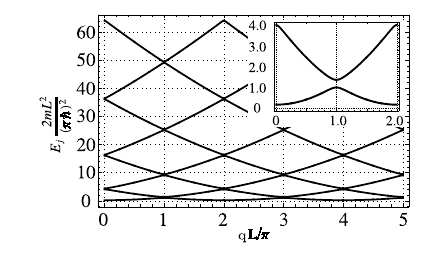
\includegraphics[ scale = 0.7]{criss-cross.png}
\end{center}\vspace*{-10pt}\caption{Energy and angular momentum of each particle. With a barrier present, there is an avoided crossing, as shown in the inset. \cite{CROSSING} }
\end{figure}

%-------------------------------------------------------------------------------
% RESOURCES
%-------------------------------------------------------------------------------

\subsection*{Resources}
As this project is theoretical in nature, the only resource requirement will be computation time. Extensive use of the high performance computing (HPC) systems
at OIST shall be employed, with special interest in the use of graphics processing units (GPU) for developing high performance numerical routines.

\begin{thebibliography}{99} % Bibliography - this is intentionally simple in this template

\bibitem[1]{CRAB} T. Caneva; T. Calarco; S. Mantangero (2011).
    \newblock Chopped random-basis quantum optimization.
    \newblock{\em Phys. Rev. A}, 84:022326.
\vspace*{-10pt}
\bibitem[2]{RING} D. Hallwood; T. Ernst; J. Brand (2010).
    \newblock Robust mesoscopic superposition of strongly correlated ultracold atoms.
    \newblock {\em Phys. Rev. A}, 82:063623.
\vspace*{-10pt}
\bibitem[3]{CROSSING} C. Shenke; A. Minguzzi; F. Hekking (2012).
    \newblock Probing superfluidity of a mesoscopic Tonks-Girardeau gas.
    \newblock {\em Phys. Rev. A}, 85:053627.
\end{thebibliography}



\end{document}